\documentclass[12pt,a4paper]{article}

\usepackage[top=2.5cm,bottom=2.5cm,left=2.5cm,right=2.5cm]{geometry}
\usepackage{mathptmx}
\usepackage{graphicx}
\usepackage{float}
\usepackage{booktabs}
\usepackage{xcolor}
\usepackage{amsmath}
\usepackage{setspace}
\usepackage{indentfirst}
\usepackage{caption}
\usepackage{titlesec}
\usepackage[hidelinks]{hyperref}
\usepackage{xurl}

\onehalfspacing
\setlength{\parindent}{1cm}
\emergencystretch=2em

\captionsetup[figure]{name=Gambar, labelsep=period, labelfont=bf, font=footnotesize, justification=centering}
\captionsetup[table]{name=Tabel, labelsep=period, labelfont=bf, font=footnotesize, justification=centering}

\titleformat{\section}
{\normalfont\fontsize{14pt}{17pt}\bfseries}
{\thesection}{0.5em}{\MakeUppercase}

\titleformat{\subsection}
{\normalfont\fontsize{12pt}{15pt}\bfseries}
{\thesubsection}{0.5em}{}

\titlespacing*{\section}{0pt}{1.2em}{0.6em}
\titlespacing*{\subsection}{0pt}{0.8em}{0.4em}

\begin{document}
	
	\hypersetup{pageanchor=false}
	\begin{titlepage}
		\centering
		\vspace*{0.2cm}
		
		{\fontsize{16pt}{20pt}\selectfont \textbf{LAPORAN PROGRES}}\\[0.2cm]
		{\fontsize{16pt}{20pt}\selectfont \textbf{SISTEM E-NOSE BERBASIS TINYML DAN CLOUD IOT}}\\[0.6cm]
		
		{\fontsize{14pt}{18pt}\selectfont \textbf{TUGAS BESAR MATA KULIAH TEKNOLOGI IOT}}\\[1.0cm]
		
		{\fontsize{12pt}{15pt}\selectfont \textbf{Dosen Pengampu: Ahmad Radhy, S.Si., M.Si.}}\\[1.2cm]
		
		
\includegraphics[width=0.33\textwidth]{logo_its.png}\\[1.2cm]
		
		{\fontsize{12pt}{15pt}\selectfont \textbf{Disusun oleh:}}\\[0.3cm]
		{\fontsize{12pt}{15pt}\selectfont
			\begin{tabular}{ll}
				Ilham Zain Muttaqin & 2042241003 \\
				Ahmad Fauzi Abdul Razzaq & 2042241017 \\
			\end{tabular}
		}\\[1.6cm]
		
		{\fontsize{14pt}{18pt}\selectfont \textbf{PRODI D4 TEKNOLOGI REKAYASA INSTRUMENTASI}}\\[0.15cm]
		{\fontsize{14pt}{18pt}\selectfont \textbf{DEPARTEMEN TEKNIK INSTRUMENTASI}}\\[0.15cm]
		{\fontsize{14pt}{18pt}\selectfont \textbf{FAKULTAS VOKASI}}\\[0.15cm]
		{\fontsize{14pt}{18pt}\selectfont \textbf{INSTITUT TEKNOLOGI SEPULUH NOPEMBER}}\\[0.15cm]
		{\fontsize{14pt}{18pt}\selectfont \textbf{SURABAYA}}\\[0.15cm]
		{\fontsize{14pt}{18pt}\selectfont \textbf{2026}}
	\end{titlepage}
	\hypersetup{pageanchor=true}
	
	\newpage
	\pagenumbering{arabic}
	
	\section{Deskripsi Sistem dan Skema Kolaborasi Proyek}
	Tugas besar pada mata kuliah Teknologi IoT ini merupakan proyek kolaborasi lintas kelas, yakni antara Kelas C (tim kami) dan Kelas A sebagai rekan kerja sama. Pembagian tanggung jawab disepakati secara berimbang: Kelas A bertugas merealisasikan perangkat keras berupa modul sensor gas beserta chamber pengujiannya, sedangkan tugas utama kami di Kelas C adalah merancang dan membangun arsitektur Cloud System menyeluruh beserta antarmuka penggunanya.
	
	Dalam perancangan antarmuka visual, dosen pengampu memberikan kebebasan implementasi berbasis web maupun aplikasi desktop, namun memberikan batasan mutlak bahwa sistem perangkat lunak wajib dibangun menggunakan bahasa pemrograman Rust. Kami memilih membangun aplikasi desktop visual menggunakan framework grafis egui (eframe) di Rust karena keunggulannya dalam aspek efisiensi memori, konkurensi thread yang aman dari race condition, serta kecepatan rendering natively. Selain antarmuka pemantauan data, dosen pengampu menetapkan dua persyaratan sistem tingkat lanjut yang wajib kami integrasikan, yaitu:
	\begin{enumerate}
		\item Modul Firmware OTA nirkabel untuk mengirimkan berkas biner firmware pembaruan langsung ke mikrokontroler melalui protokol MQTT.
		\item Fitur Active Learning berbasis Ingestion API menuju platform Edge Impulse, di mana operator dapat memvalidasi prediksi model dan secara otomatis mengunggah data misclassified ke dataset cloud untuk keperluan pelatihan ulang model secara adaptif.
	\end{enumerate}
	
	\section{Perancangan Alat Peraga Pengujian Perangkat Keras}
	Mengingat pengerjaan perangkat keras sensor gas oleh Kelas A belum sepenuhnya tuntas, kami berinisiatif merancang alat peraga pengujian mandiri pada breadboard. Tujuannya adalah memastikan seluruh pipeline sistem yang kami bangun mulai dari akuisisi ADC, inferensi Edge AI, transmisi MQTT TLS, eksekusi Active Learning, hingga pembaruan Firmware OTA dapat diuji dan dievaluasi fungsionalitasnya secara presisi tanpa harus terhambat oleh keterlambatan penyelesaian hardware fisik.
	
	\begin{figure}[H]
		\centering
		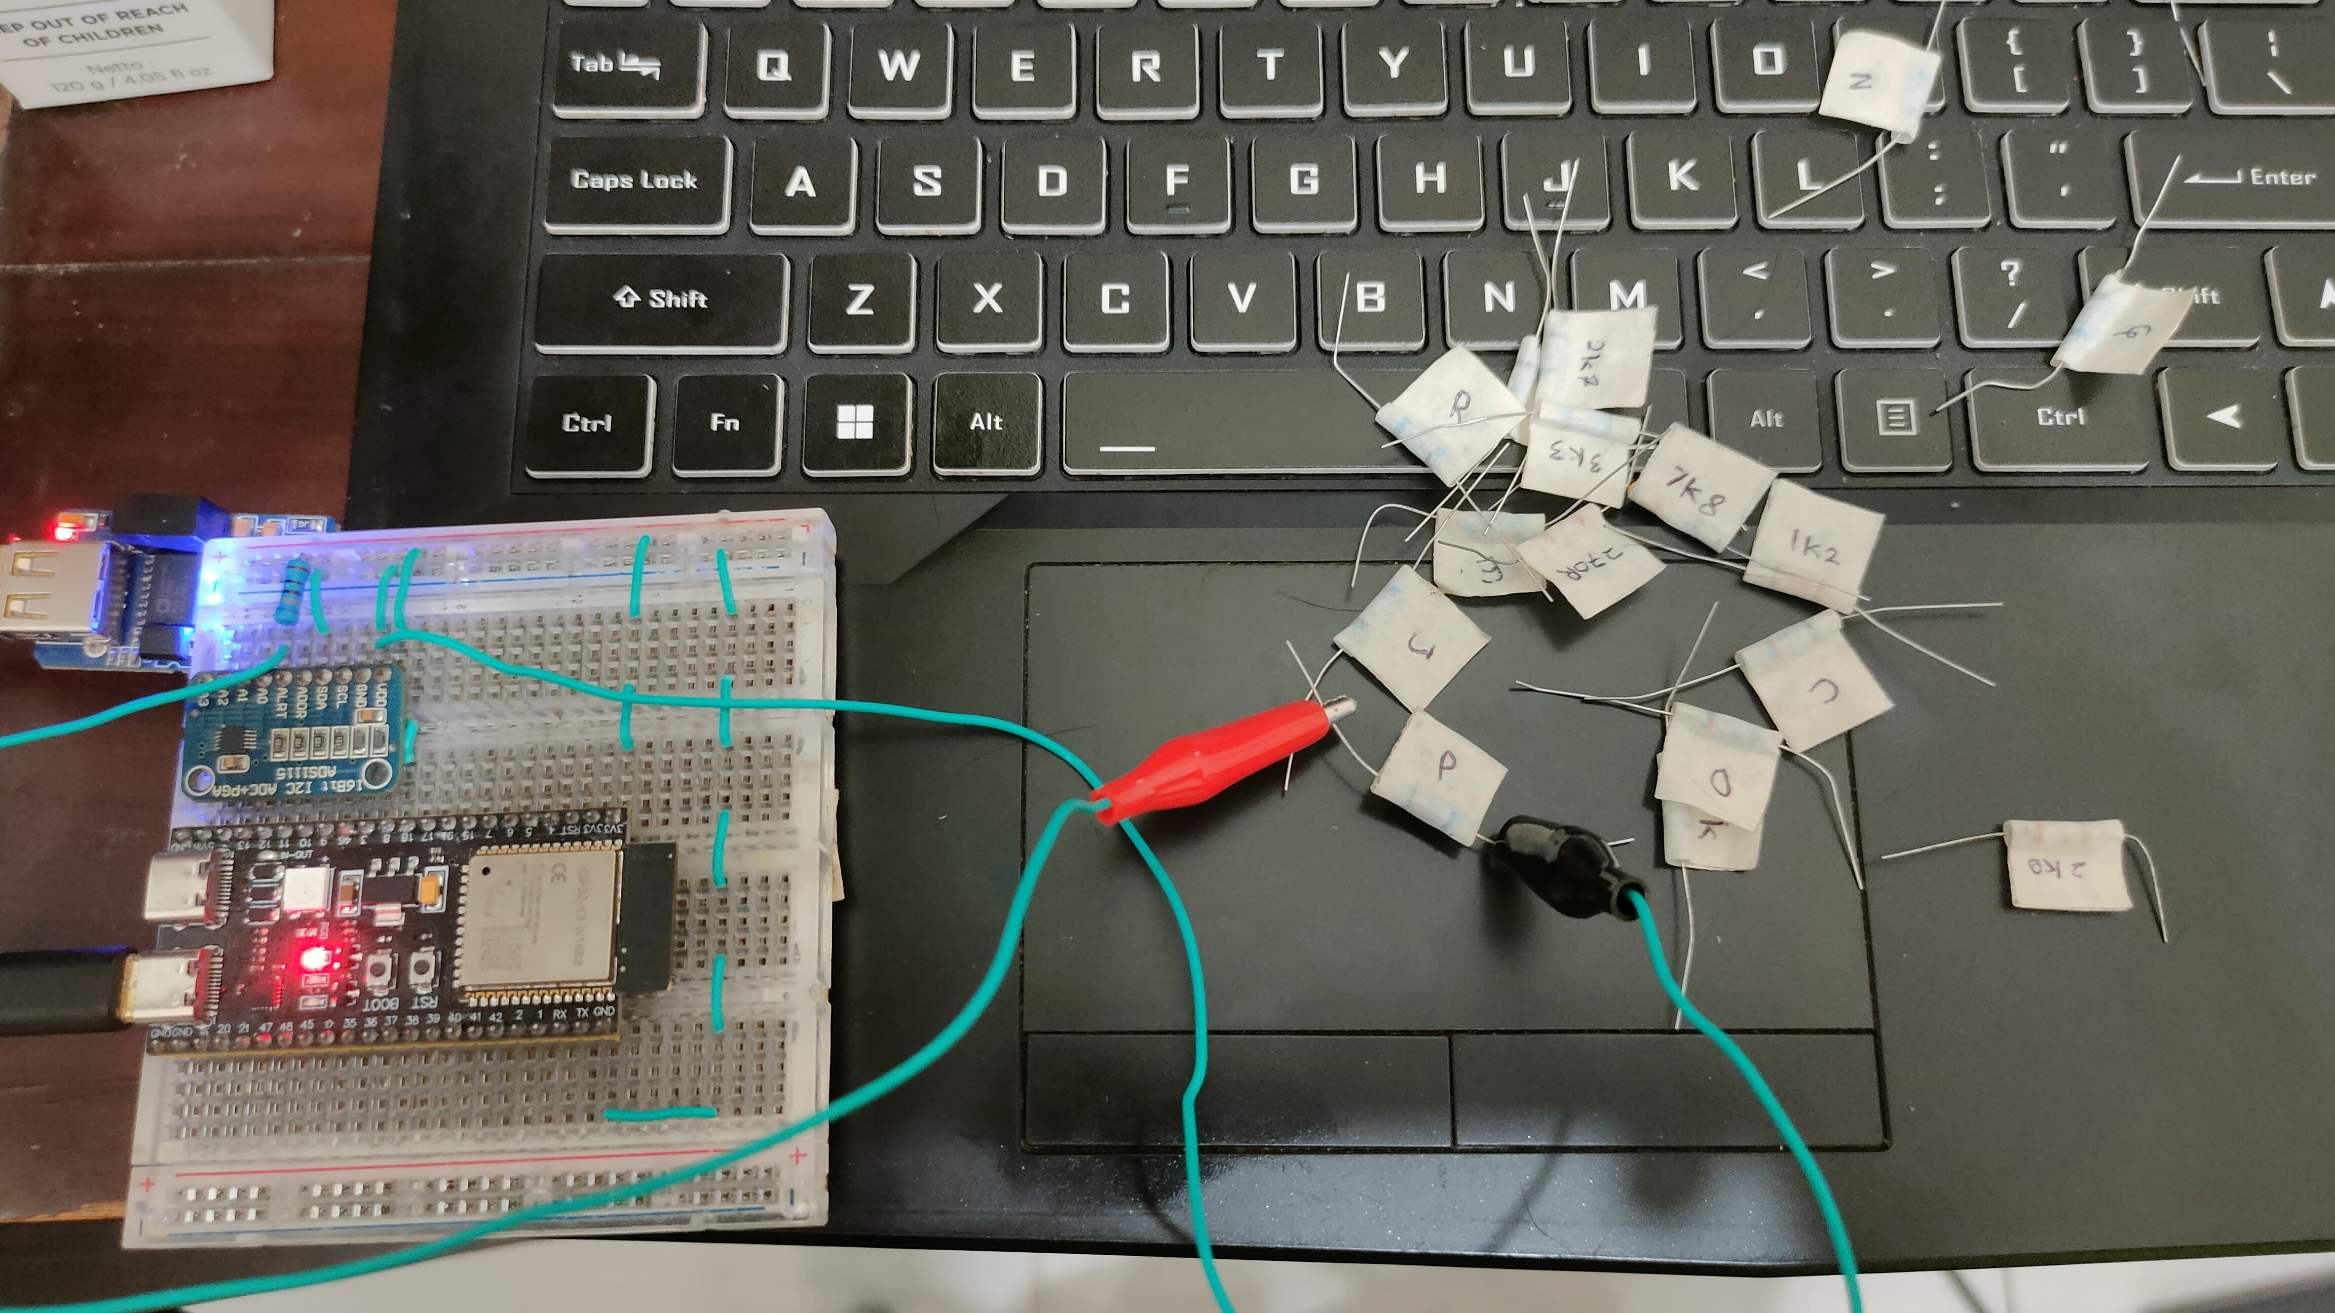
\includegraphics[width=0.82\textwidth]{gambar1_hardware.png}
		\caption{Alat peraga pengujian perangkat keras pada breadboard memuat ESP32-S3, modul ADS1115, dan resistor pembagi tegangan sebanyak 18 sampel.}
	\end{figure}
	
	Alat peraga ini kami bangun menggunakan mikrokontroler ESP32-S3 dan modul Analog-to-Digital Converter eksternal ADS1115 berkemampuan 16-bit melalui jalur komunikasi I2C pada pin GPIO 8 (SDA) dan GPIO 9 (SCL). Kami mengatur penguatan internal ADS1115 pada mode Gain 1 (skala penuh $\pm 4,096\text{ V}$) dengan alamat I2C default 0x48. Pada kanal A0, kami merancang sirkuit pembagi tegangan dengan resistor tetap $R_1$ sebesar $680\ \Omega$ bertoleransi presisi 1\% yang terhubung ke rel tegangan teregulasi $3,3\text{ V}$. 
	
	Resistor beban $R_2$ kami pasang modular menggunakan 18 nilai hambatan berbeda yang mewakili 18 jenis sampel aroma volatil (Sample\_A hingga Sample\_R). Nilai tegangan keluaran analog dihitung berdasarkan persamaan:
	\begin{equation}
		V_{\text{out}} = 3,3\text{ V} \times \frac{R_2}{680\ \Omega + R_2}
	\end{equation}
	
	Tegangan analog terukur dikonversi menjadi angka normalisasi desimal $0,0$ hingga $1,0$. Nilai ini kemudian dimasukkan secara simultan ke dalam 10 sumbu kanal sensor instrumen analitik, yaitu MQ3, MQ7, MQ135, MQ6, TGS2600, TGS2602, TGS2611, TGS2620, DHT\_Temp, dan DHT\_Hum pada frekuensi sampling stabil 50 Hz (interval 20 milidetik non-blocking). Rincian toleransi resistor dan profil nilai terukur disajikan pada Tabel 1.
	
	\begin{table}[H]
		\centering
		\begin{tabular}{ccccc}
			\toprule
			\textbf{Label Sampel} & \textbf{Resistor $R_1$} & \textbf{Resistor $R_2$} & \textbf{Tegangan $V_{\text{out}}\ (\text{V})$} & \textbf{Nilai Normalisasi} \\
			\midrule
			Sample\_A & 680 $\Omega$ (1\%) & 220 $\Omega$ (5\%) & 0,807 & 0,244 \\
			Sample\_B & 680 $\Omega$ (1\%) & 270 $\Omega$ (5\%) & 0,938 & 0,284 \\
			Sample\_C & 680 $\Omega$ (1\%) & 300 $\Omega$ (1\%) & 1,010 & 0,306 \\
			Sample\_D & 680 $\Omega$ (1\%) & 330 $\Omega$ (5\%) & 1,078 & 0,327 \\
			Sample\_E & 680 $\Omega$ (1\%) & 470 $\Omega$ (5\%) & 1,349 & 0,409 \\
			Sample\_F & 680 $\Omega$ (1\%) & 560 $\Omega$ (1\%) & 1,490 & 0,452 \\
			Sample\_G & 680 $\Omega$ (1\%) & 820 $\Omega$ (5\%) & 1,804 & 0,547 \\
			Sample\_H & 680 $\Omega$ (1\%) & 1,0 k$\Omega$ (5\%) & 1,964 & 0,595 \\
			Sample\_I & 680 $\Omega$ (1\%) & 1,2 k$\Omega$ (5\%) & 2,106 & 0,638 \\
			Sample\_J & 680 $\Omega$ (1\%) & 2,2 k$\Omega$ (5\%) & 2,521 & 0,764 \\
			Sample\_K & 680 $\Omega$ (1\%) & 2,7 k$\Omega$ (5\%) & 2,636 & 0,799 \\
			Sample\_L & 680 $\Omega$ (1\%) & 2,9 k$\Omega$ (5\%) & 2,673 & 0,810 \\
			Sample\_M & 680 $\Omega$ (1\%) & 3,3 k$\Omega$ (5\%) & 2,736 & 0,829 \\
			Sample\_N & 680 $\Omega$ (1\%) & 4,7 k$\Omega$ (5\%) & 2,883 & 0,874 \\
			Sample\_O & 680 $\Omega$ (1\%) & 5,6 k$\Omega$ (5\%) & 2,943 & 0,892 \\
			Sample\_P & 680 $\Omega$ (1\%) & 6,8 k$\Omega$ (1\%) & 2,999 & 0,909 \\
			Sample\_Q & 680 $\Omega$ (1\%) & 7,8 k$\Omega$ (5\%) & 3,035 & 0,920 \\
			Sample\_R & 680 $\Omega$ (1\%) & 10,0 k$\Omega$ (5\%) & 3,090 & 0,936 \\
			\bottomrule
		\end{tabular}
		\vspace{0.2cm}
		\caption{Daftar nilai hambatan simulasi sampel gas A sampai R pada kanal A0.}
	\end{table}
	
	\section{Arsitektur Cloud MQTT dan Desktop GUI Berbasis Rust}
	Infrastruktur transmisi data nirkabel dibangun menggunakan protokol MQTT terenkripsi TLS pada port 8883 menuju broker HiveMQ Cloud di alamat host serverless \nolinkurl{84aec46d41534b009368ec20fc74362c.s1.eu.hivemq.cloud}. Autentikasi sesi klien dibagi menjadi dua akun tersendiri, yaitu akun \texttt{hardware\_side} untuk mikrokontroler dan akun \texttt{software\_side} untuk aplikasi desktop guna menjamin kontrol akses yang terisolasi.
	
	\begin{figure}[H]
		\centering
		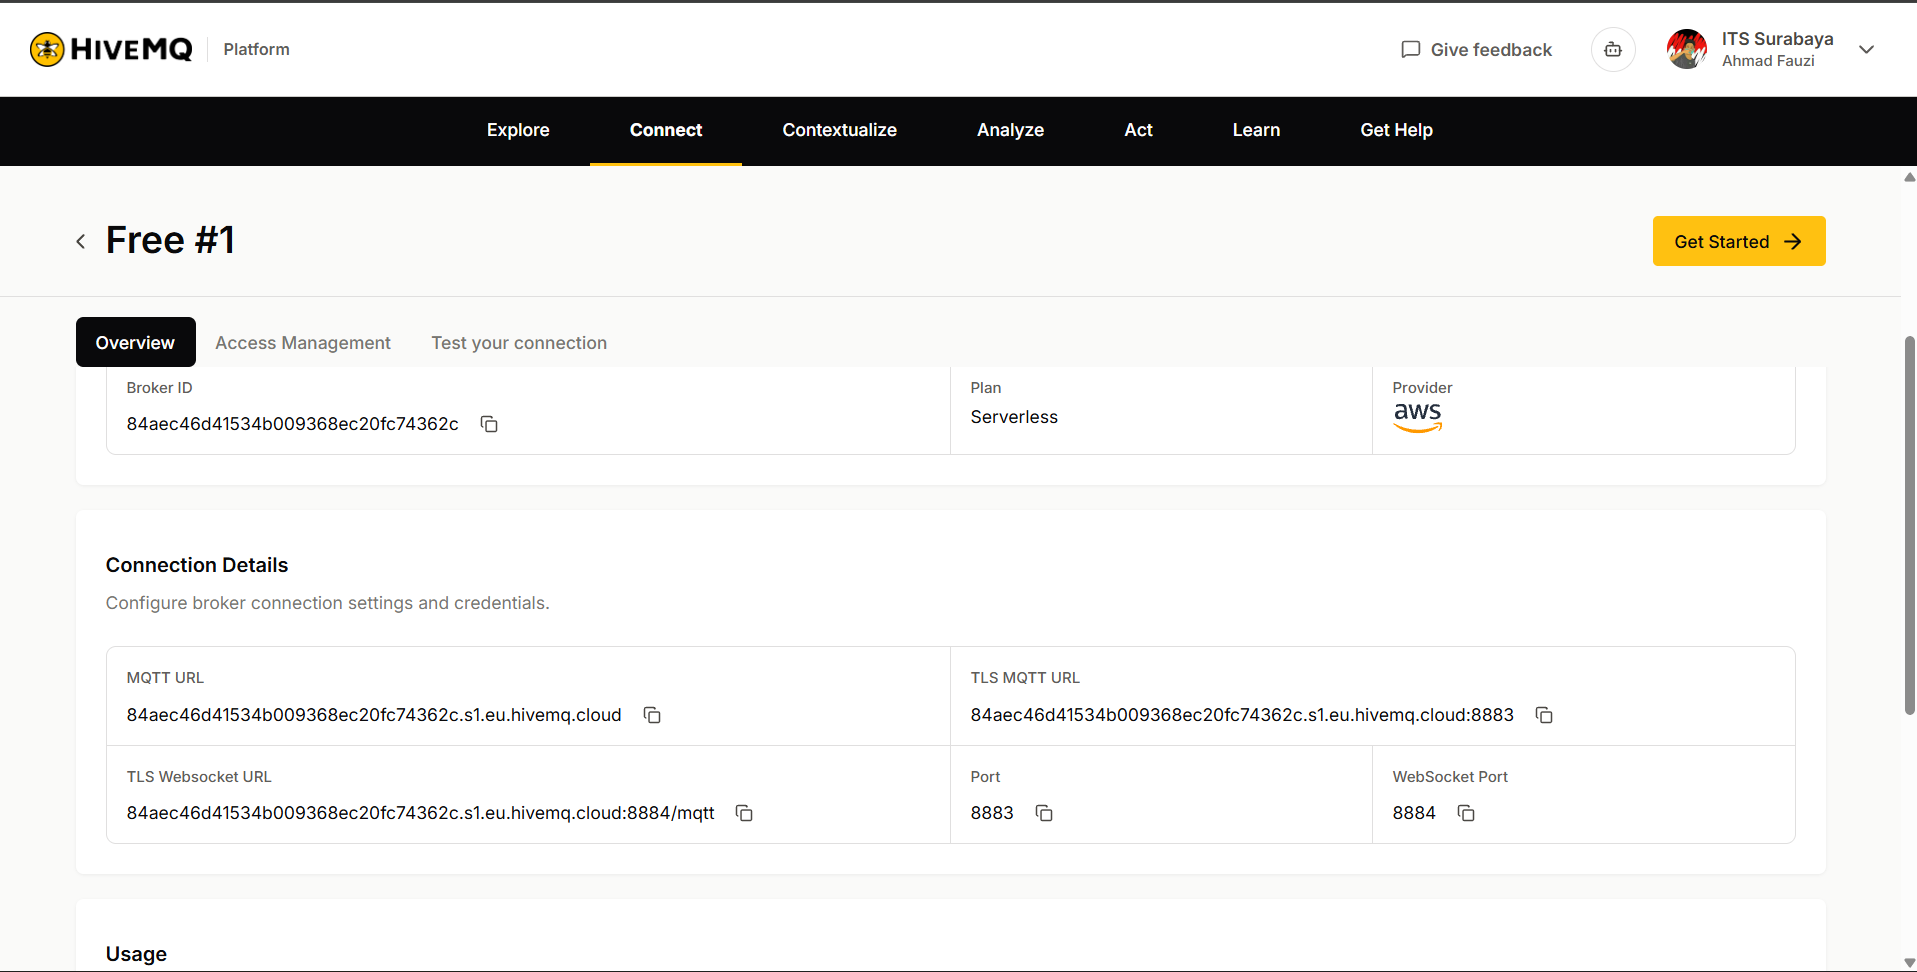
\includegraphics[width=0.88\textwidth]{gambar2_hivemq.png}
		\caption{Dasbor kluster serverless HiveMQ Cloud yang aktif mengelola koneksi MQTTS port 8883.}
	\end{figure}
	
	Aplikasi desktop GUI E-Nose dirancang menggunakan bahasa pemrograman Rust dengan framework grafis \texttt{eframe}. Kami menerapkan arsitektur multithread di mana soket jaringan dikelola oleh crate \texttt{rumqttc} pada thread latar belakang, sementara thread visual utama bertugas merender antarmuka bertema industrial dark mode pada resolusi terkunci 1920x1080 piksel (dengan dukungan mode layar penuh melalui pintasan keyboard F11). Komunikasi antar thread dijembatani secara aman menggunakan kanal asinkron \texttt{std::sync::mpsc}.
	
	\begin{figure}[H]
		\centering
		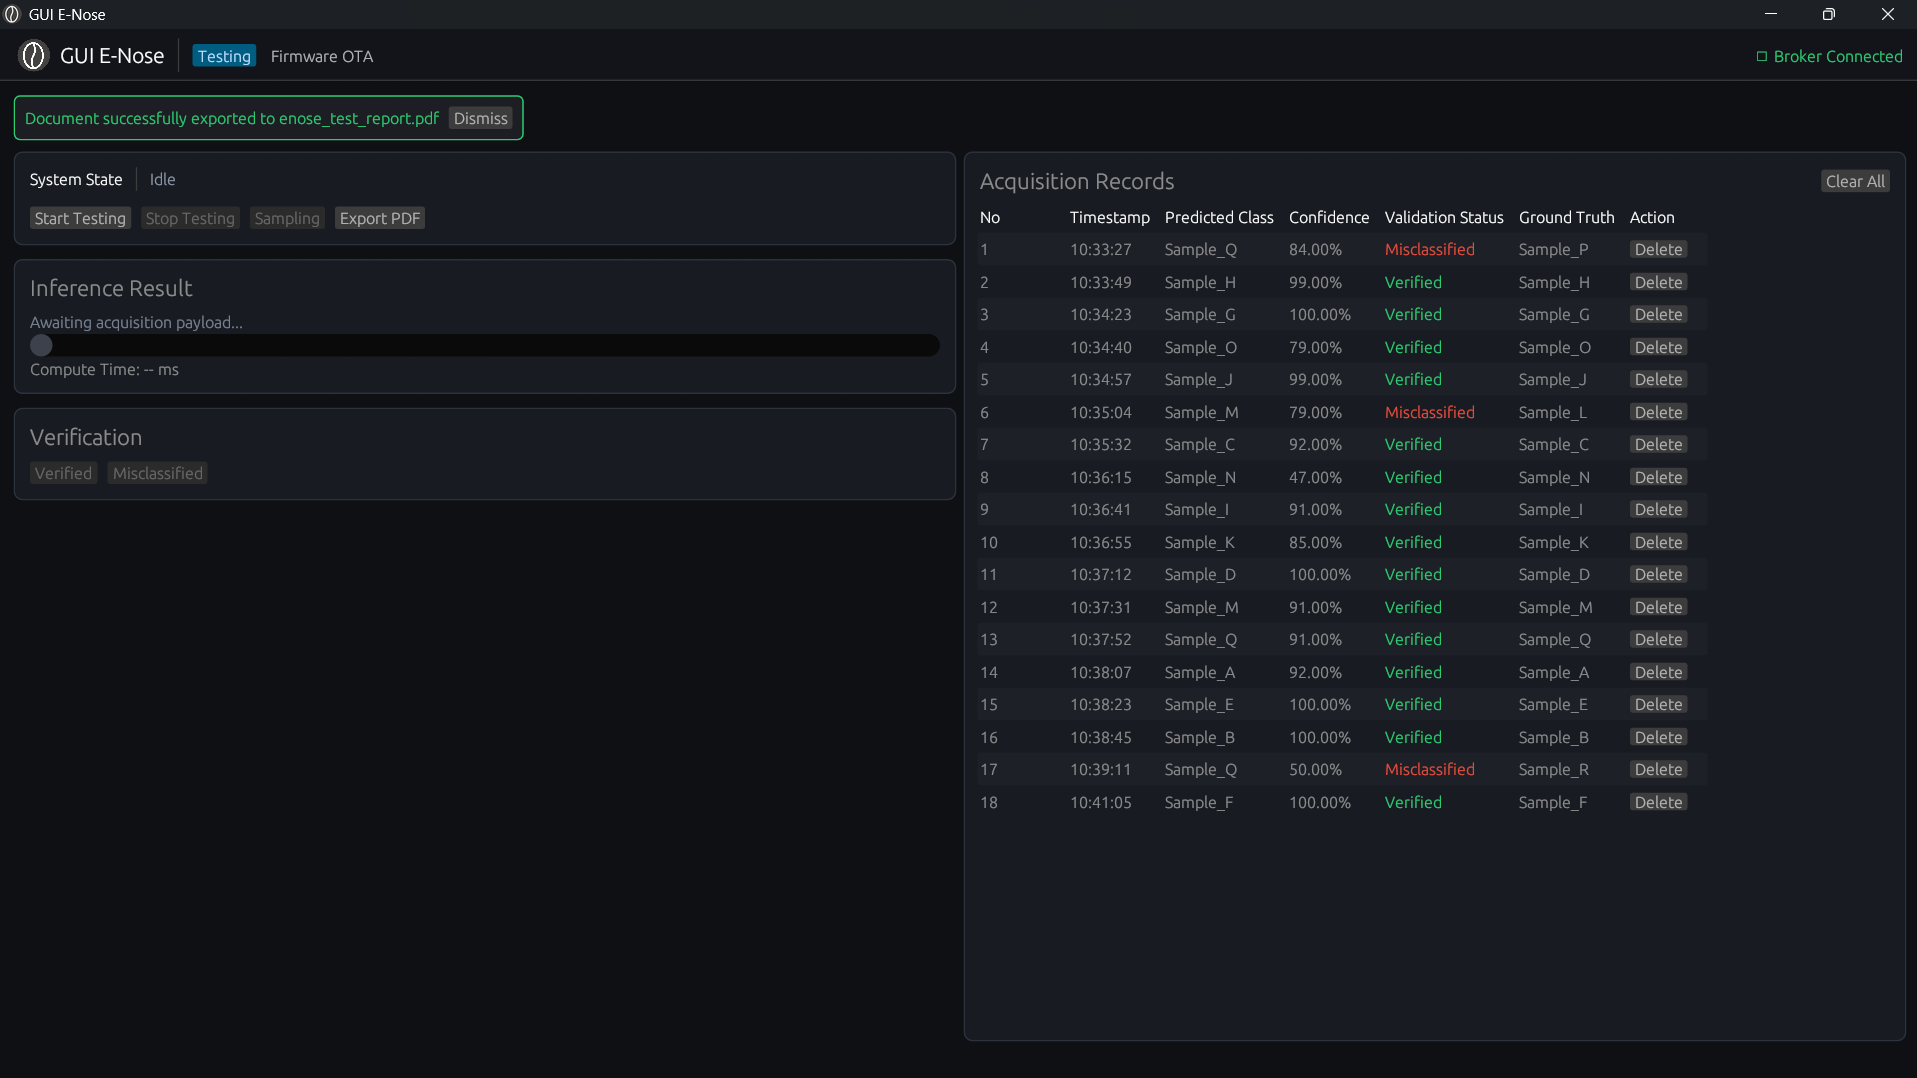
\includegraphics[width=0.92\textwidth]{gambar3_gui_testing.png}
		\caption{Tampilan antarmuka desktop GUI E-Nose pada tab Testing dengan panel State Machine, hasil inferensi, dan tabel Acquisition Records.}
	\end{figure}
	
	Alur operasional pengujian dikunci secara ketat menggunakan Finite State Machine berbasis tipe data enum dengan empat status: Idle, Testing, Sampling, dan Verification. Tombol sampling hanya aktif saat sistem berada pada status Testing. Ketika ditekan, GUI mengirim instruksi ke topik \texttt{esp32/cmd/sampling} dan mengunci tombol sampling dalam status hold dengan batas timeout 10 detik. Jika mikrokontroler tidak merespons dalam jendela waktu tersebut, antarmuka memunculkan banner peringatan dan secara aman membuka kembali sistem ke mode siaga.
	
	Pada tabel Acquisition Records, hasil pengujian dicatat secara berurutan. Kami menambahkan fitur manajemen data berupa tombol delete individual per baris rekaman serta tombol clear all sehingga operator dapat mereset data pengujian secara dinamis tanpa perlu merestart aplikasi.
	
	\section{Implementasi Protokol Firmware OTA Nirkabel}
	Guna memenuhi instruksi dosen mengenai pemeliharaan firmware jarak jauh, kami menyediakan tab Firmware OTA pada antarmuka desktop. Pengguna dapat memilih berkas biner \texttt{.bin} hasil kompilasi Arduino IDE menggunakan pemilih berkas native berbasis crate \texttt{rfd}.
	
	\begin{figure}[H]
		\centering
		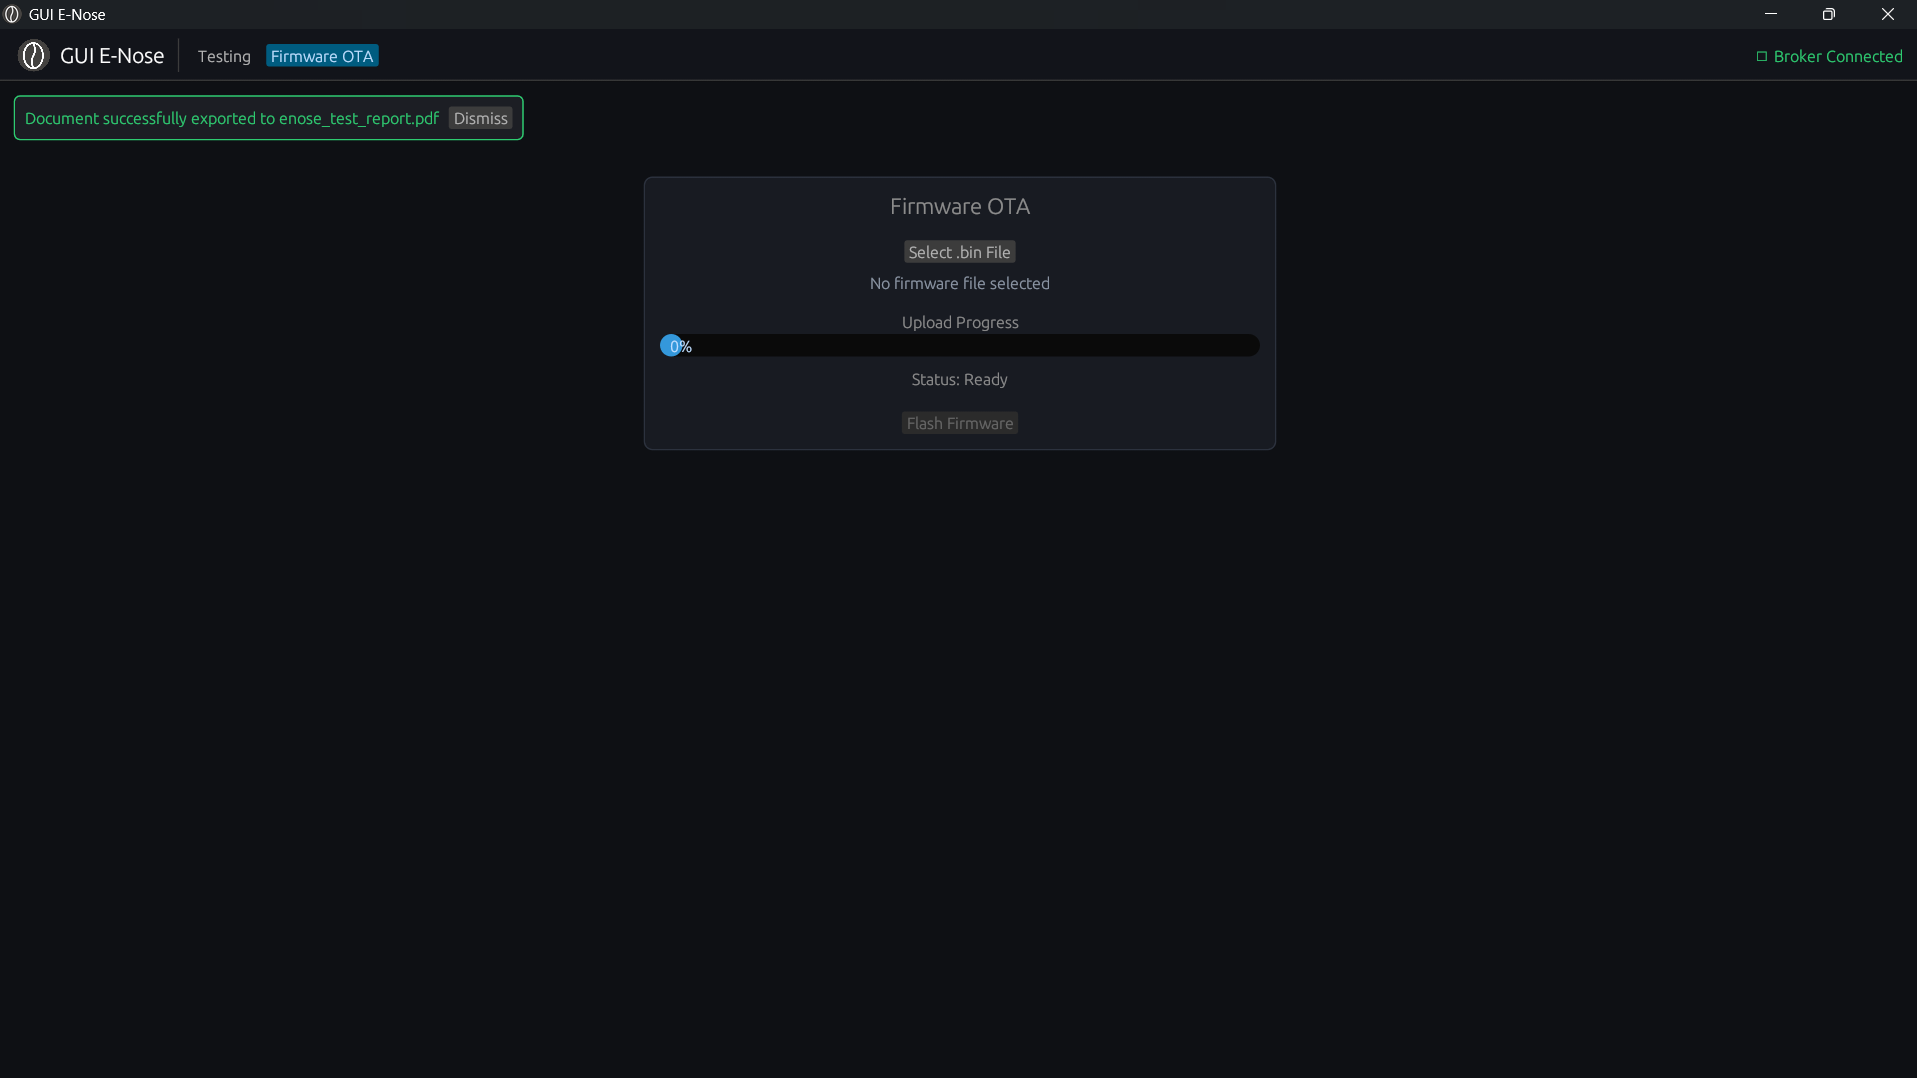
\includegraphics[width=0.92\textwidth]{gambar4_gui_ota.png}
		\caption{Tampilan antarmuka desktop GUI E-Nose pada tab Firmware OTA saat kondisi siaga instalasi firmware.}
	\end{figure}
	
	Saat proses flashing dieksekusi, thread transmisi memecah file biner menjadi paket-paket berukuran 1024 byte, mengirimkannya secara berurutan ke topik \texttt{esp32/ota/payload} dengan QoS 0, dan menunggu konfirmasi balik dari topik \texttt{esp32/ota/ack} sebelum mentransmisikan paket berikutnya. Batas timeout respons ACK diatur sebesar 15 detik untuk mengantisipasi jeda penghapusan sektor flash memori ESP32-S3 serta latensi jaringan internasional broker cloud. Selama transfer byte OTA atau pengujian aktif berlangsung, tombol navigasi perpindahan halaman dikunci otomatis guna mencegah kegagalan partisi memori.
	
	\section{Integrasi Active Learning Edge Impulse}
	Model machine learning TinyML diekspor dari platform Edge Impulse ke dalam pustaka C++ \texttt{IoT\_inferencing.h} dan ditanamkan ke dalam firmware ESP32-S3. Ketika ESP32-S3 menerima instruksi sampling, fungsi inferensi \texttt{run\_classifier} mengeksekusi ekstraksi fitur dan klasifikasi neural network. Hasil inferensi berupa label kelas dengan probabilitas tertinggi, nilai konfidensi, durasi komputasi milidetik, serta 10 data mentah sensor analog dikemas ke dalam format JSON dan dipublikasikan ke topik \texttt{esp32/data/result}.
	
	\begin{figure}[H]
		\centering
		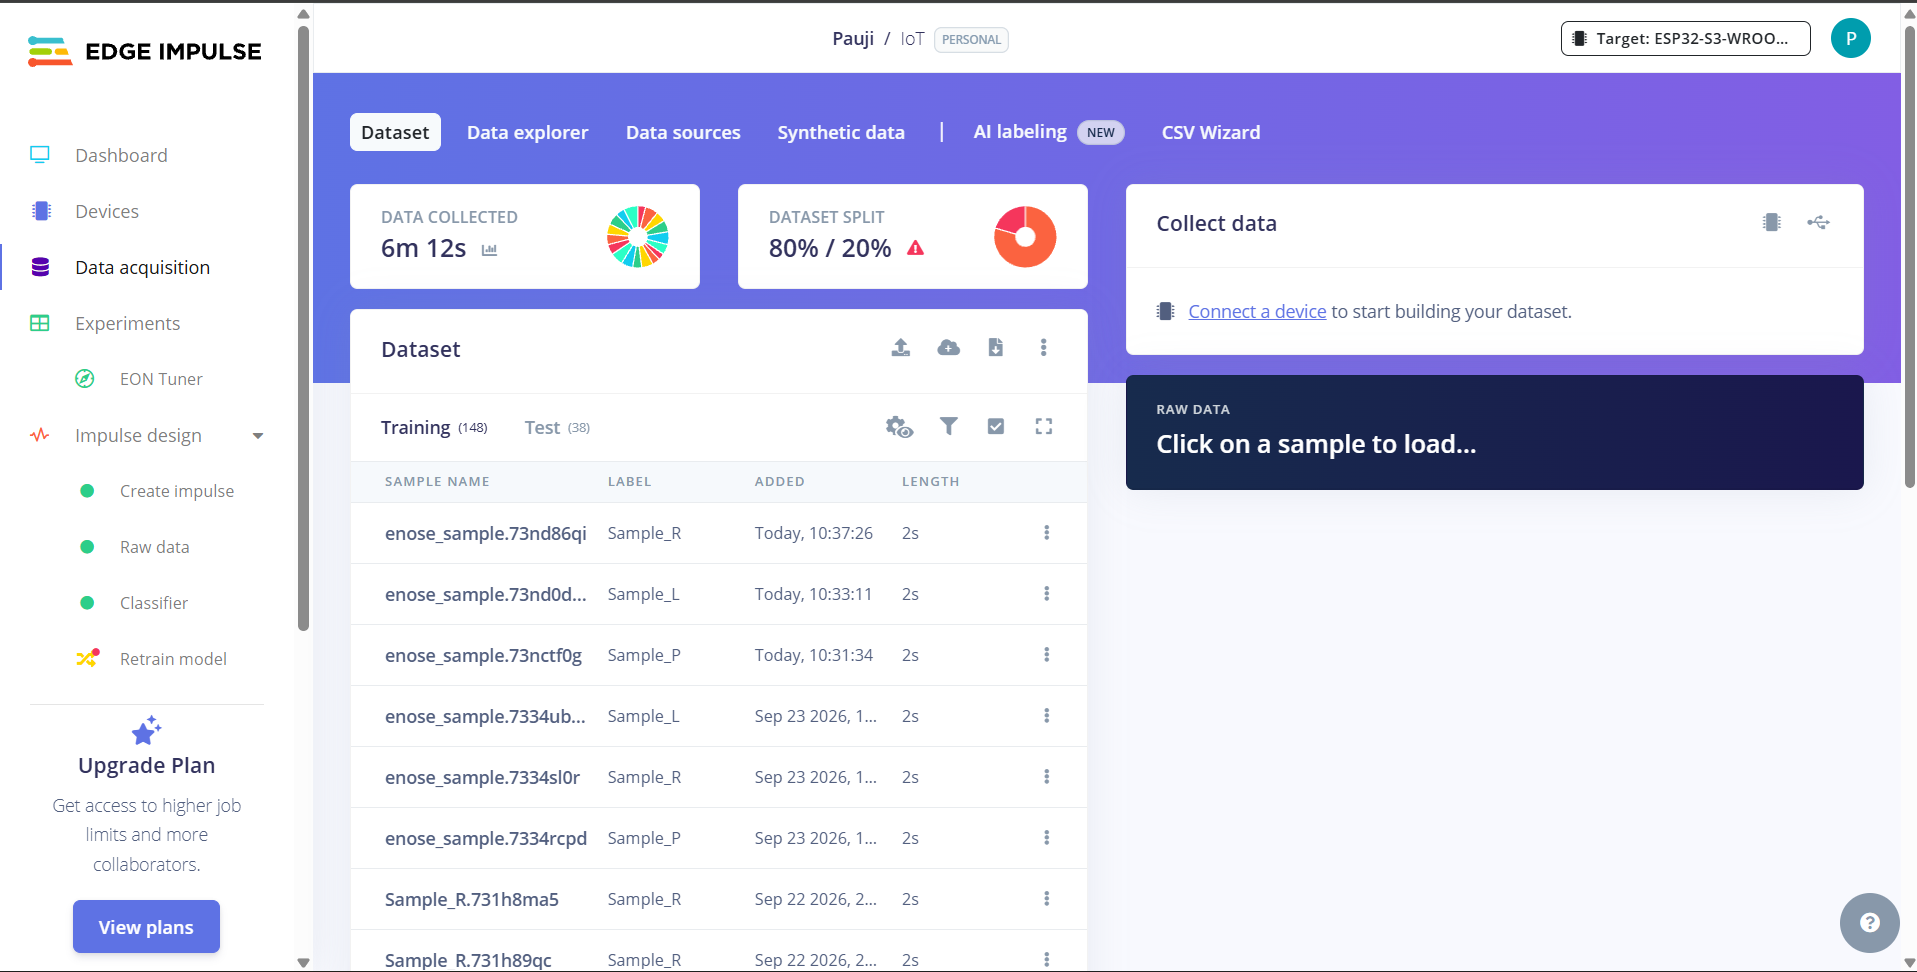
\includegraphics[width=0.92\textwidth]{gambar5_edge_impulse.png}
		\caption{Dasbor repositori Edge Impulse yang memvalidasi keberhasilan penerimaan sampel data gas dengan durasi 2 detik melalui Ingestion API.}
	\end{figure}
	
	Ketika operator mendeteksi hasil prediksi yang keliru, penekanan tombol Misclassified dan pemilihan kelas target sebenarnya dari menu dropdown memicu thread asinkron berbasis pustaka \texttt{reqwest} untuk mengirimkan data ke endpoint \url{https://ingestion.edgeimpulse.com/api/training/data}. Request dikirim menggunakan header otorisasi \texttt{x-api-key}, label koreksi pada \texttt{x-label}, serta nama berkas \texttt{enose\_sample.json}. Matriks nilai mentah disusun menjadi 100 baris perulangan dengan interval 20 milidetik untuk membentuk rekaman sampel utuh berdurasi 2 detik pada frekuensi 50 Hz. Transmisi ini terbukti berhasil memasukkan data koreksi ke dataset cloud Edge Impulse secara instan tanpa menghentikan kelancaran rendering visual antarmuka.
	
	\section{Validasi Hasil Pengujian dan Laporan Resmi PDF}
	Pada akhir sesi pengujian, sistem desktop menyediakan fitur pencetakan dokumen audit resmi berformat PDF secara native menggunakan pustaka \texttt{printpdf}. Laporan memuat identitas instrumen, tabel pengujian bergaris transparan, watermark logo tim riset HUPOMONĒ dengan tingkat transparansi 8\%, serta catatan ringkasan metrik akurasi sistem.
	
	\begin{figure}[H]
		\centering
		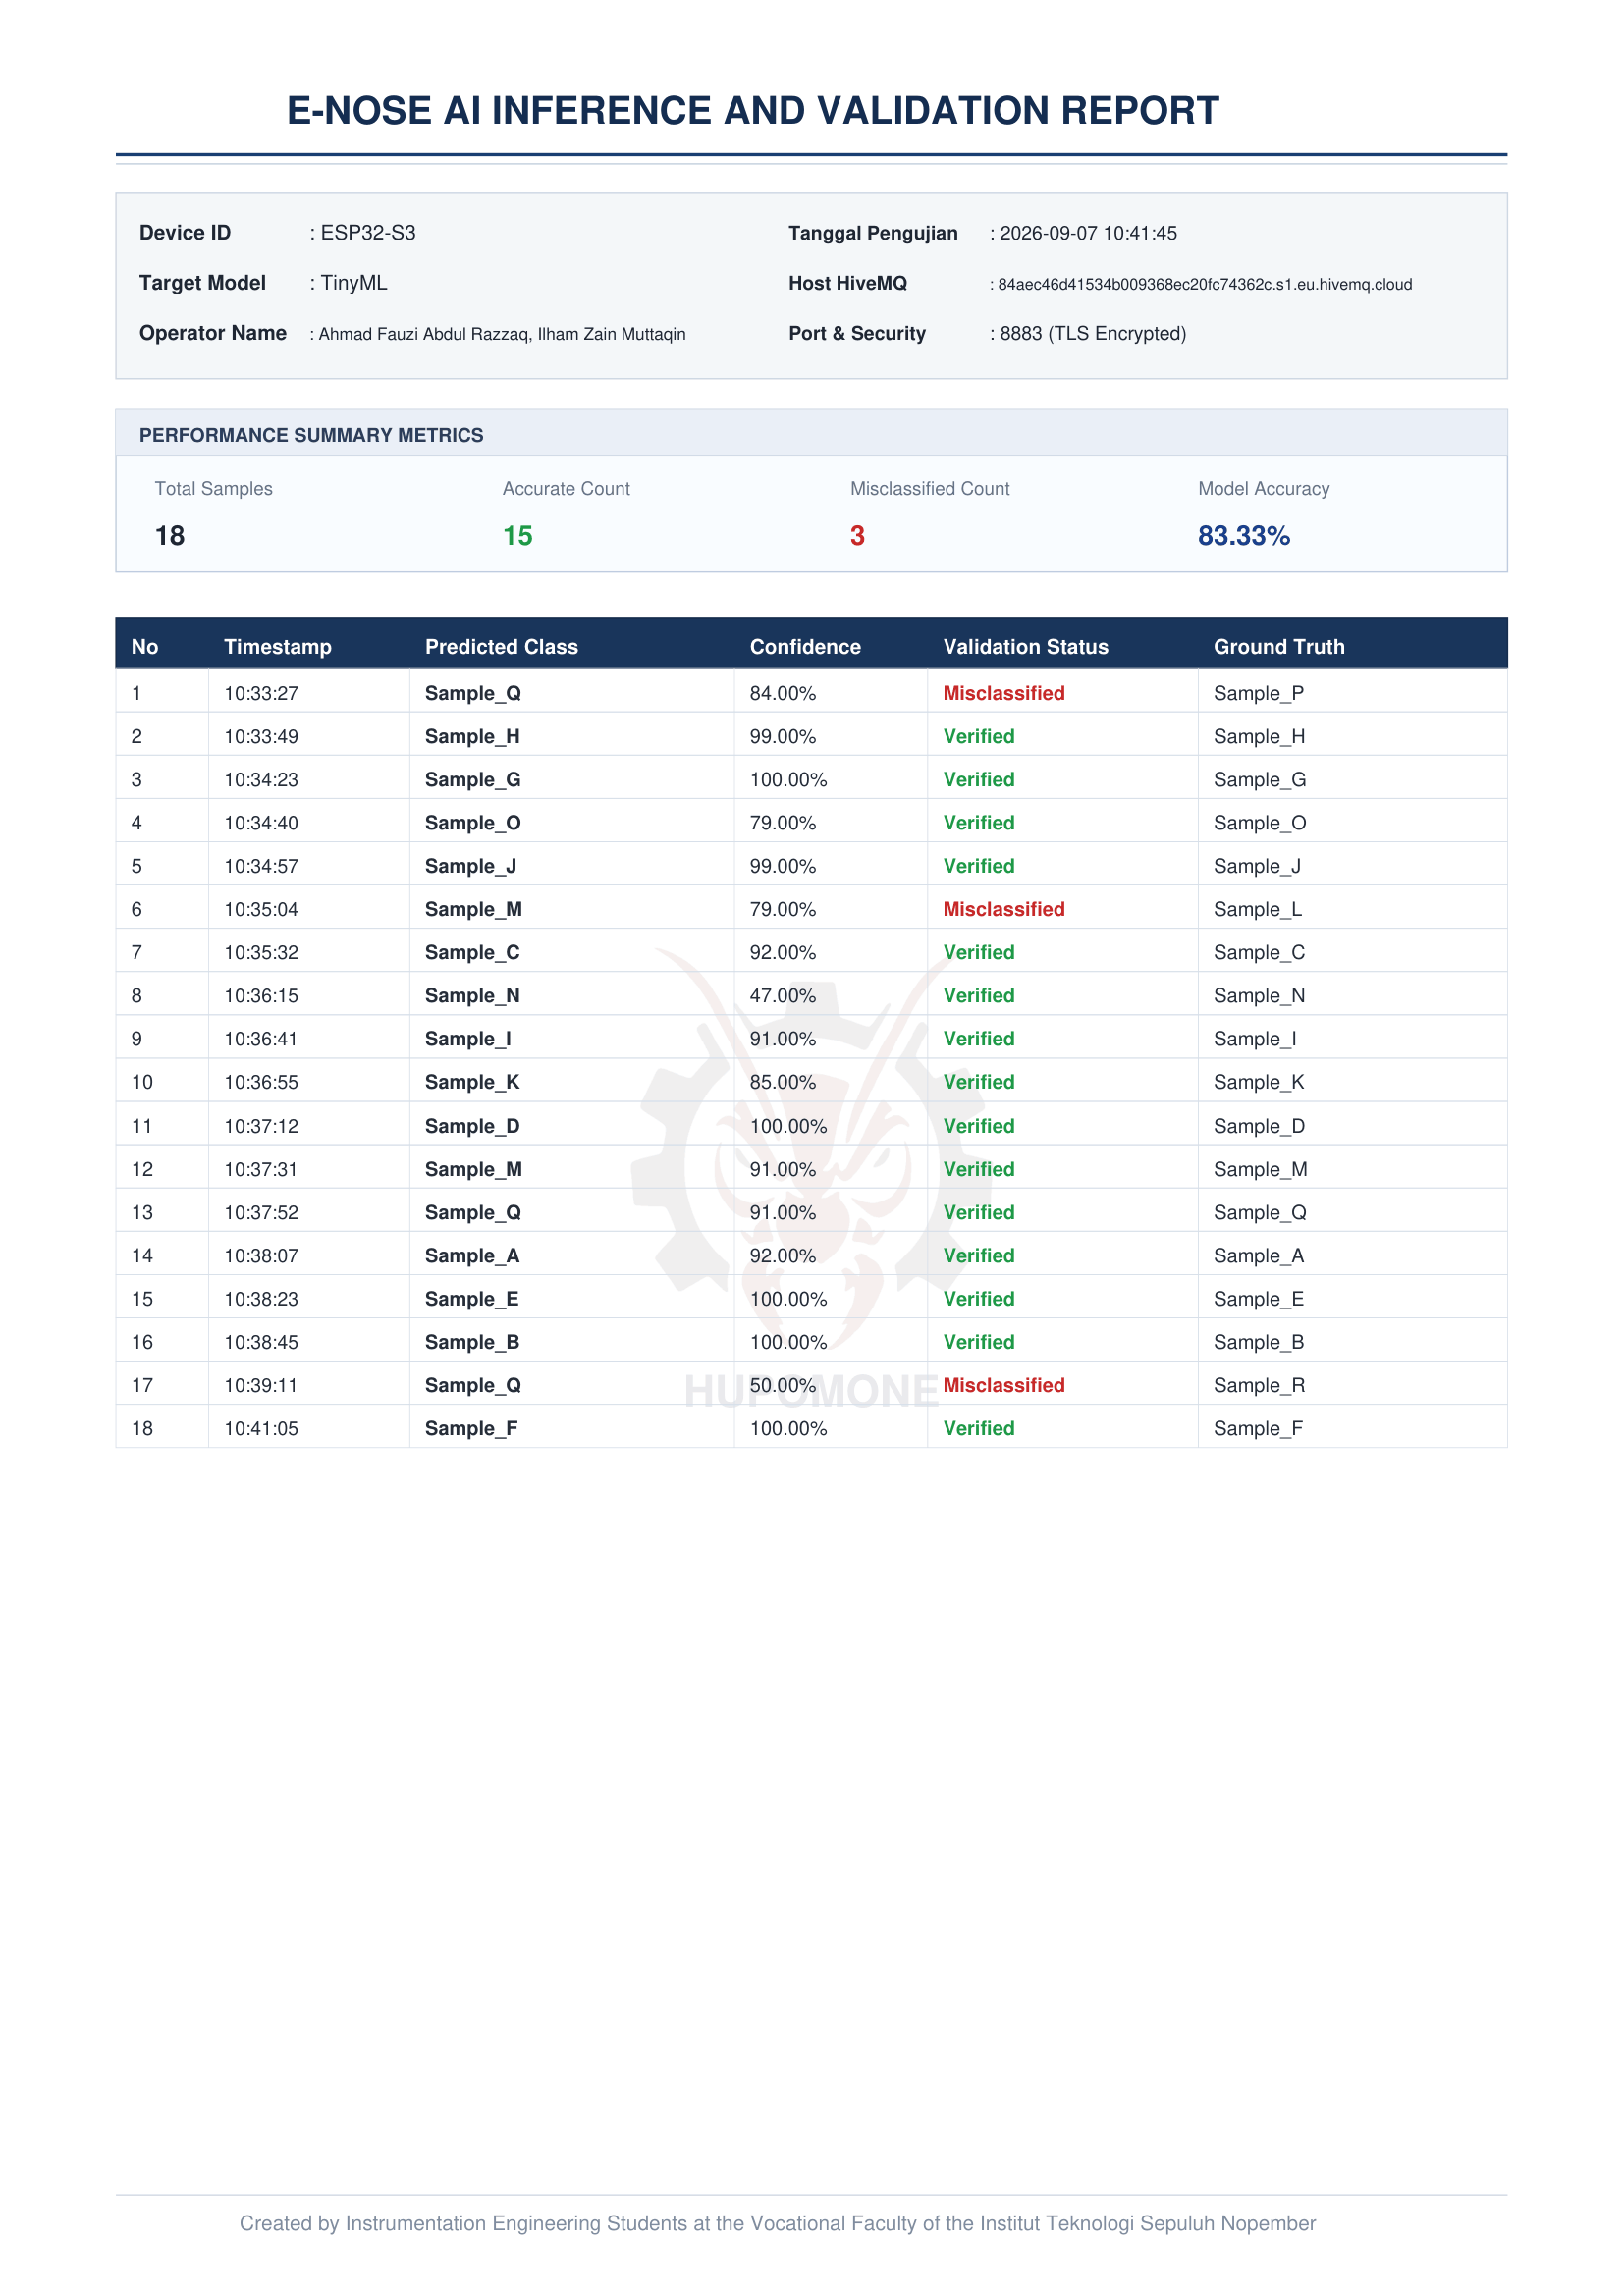
\includegraphics[width=0.78\textwidth]{gambar6_pdf_report.png}
		\caption{Dokumen laporan pengujian resmi berformat PDF ber-watermark HUPOMONĒ hasil render engine native printpdf.}
	\end{figure}
	
	Dari 18 data sampel representatif yang kami uji di laboratorium menggunakan alat peraga (Sample\_A hingga Sample\_R), model TinyML mengklasifikasikan 15 sampel secara tepat dan mencatat 3 kesalahan prediksi, sehingga menghasilkan akurasi keseluruhan sistem sebesar 83,33\% sebagaimana terekam pada laporan pengujian resmi.
	
	\section{Kesimpulan dan Progres Tahap Selanjutnya}
	Berdasarkan perancangan, implementasi, dan pengujian yang telah kami laksanakan, progres tugas besar ini telah berhasil membuktikan seluruh fungsi sistem yang menjadi tanggung jawab kami:
	\begin{enumerate}
		\item Alat peraga pengkondisi sinyal ADS1115 pada mode Gain 1 terbukti akurat dalam mengukur 18 variasi pola tegangan sensor pembagi resistor pada interval sampling stabil 20 milidetik (50 Hz).
		\item Jaringan komunikasi aman MQTT TLS port 8883 pada broker HiveMQ Cloud terbukti andal dalam menyalurkan perintah sampling, hasil inferensi, dan paket biner Firmware OTA tanpa kebocoran memori pada ESP32-S3.
		\item Aplikasi desktop GUI E-Nose berbasis Rust dengan framework egui berhasil mengunci alur operasional pengujian melalui Finite State Machine dan merender dokumen laporan PDF formal berstandar industri secara mandiri.
		\item Pipeline MLOps loop tertutup (Active Learning) berhasil direalisasikan melalui Edge Impulse Ingestion API, di mana data hasil koreksi operator otomatis terunggah ke repositori cloud untuk kebutuhan pelatihan ulang model.
		\item Pengujian model inferensi TinyML mencatatkan performa akurasi sistem riil sebesar 83,33\% dari 18 variasi kelas sampel gas.
	\end{enumerate}
	
	Tindak lanjut proyek selanjutnya adalah menunggu kesiapan modul hardware fisik dari Kelas A untuk diintegrasikan secara langsung ke dalam sistem Cloud IoT, pengayaan variasi data latih pada repositori cloud Edge Impulse guna meningkatkan akurasi klasifikasi model TinyML mendekati 95\%, serta optimasi ukuran partisi flash firmware ESP32-S3 untuk mempercepat durasi transfer biner nirkabel Firmware OTA.
	
\end{document}